\ac{COD} is one of the most essential variables in the process of a biological treatment since experts can make decisions based on the measurements of this variable. The objective of biological wastewater treatment is to remove the pollutants present in water. Thus, this treatment is used overall because it is compelling and more efficient than numerous mechanical or compound procedures. In the bioreactor at this stage, a variety of microorganisms are used to break down organic matter in the water. However, these microorganisms are susceptible to change, depending on several bioreactor conditions. Likewise, it turns out relevant monitoring the concentration of biomass available in the bioreactor, which indicates the state of the population of the microorganisms.

This study proposes to predict one-day time-window \ac{COD}\textsubscript{D}, \ac{COD}\textsubscript{EQ}, and \ac{MLVSS}, essential parameters in decision-making. Knowing how contaminated the water will be at the effluent stream (discharge point), the organic matter concentration at the input of the bioreactor, and how the microorganism population in charge of the biological stage is going to behave. 

\begin{figure}[h]
\centering
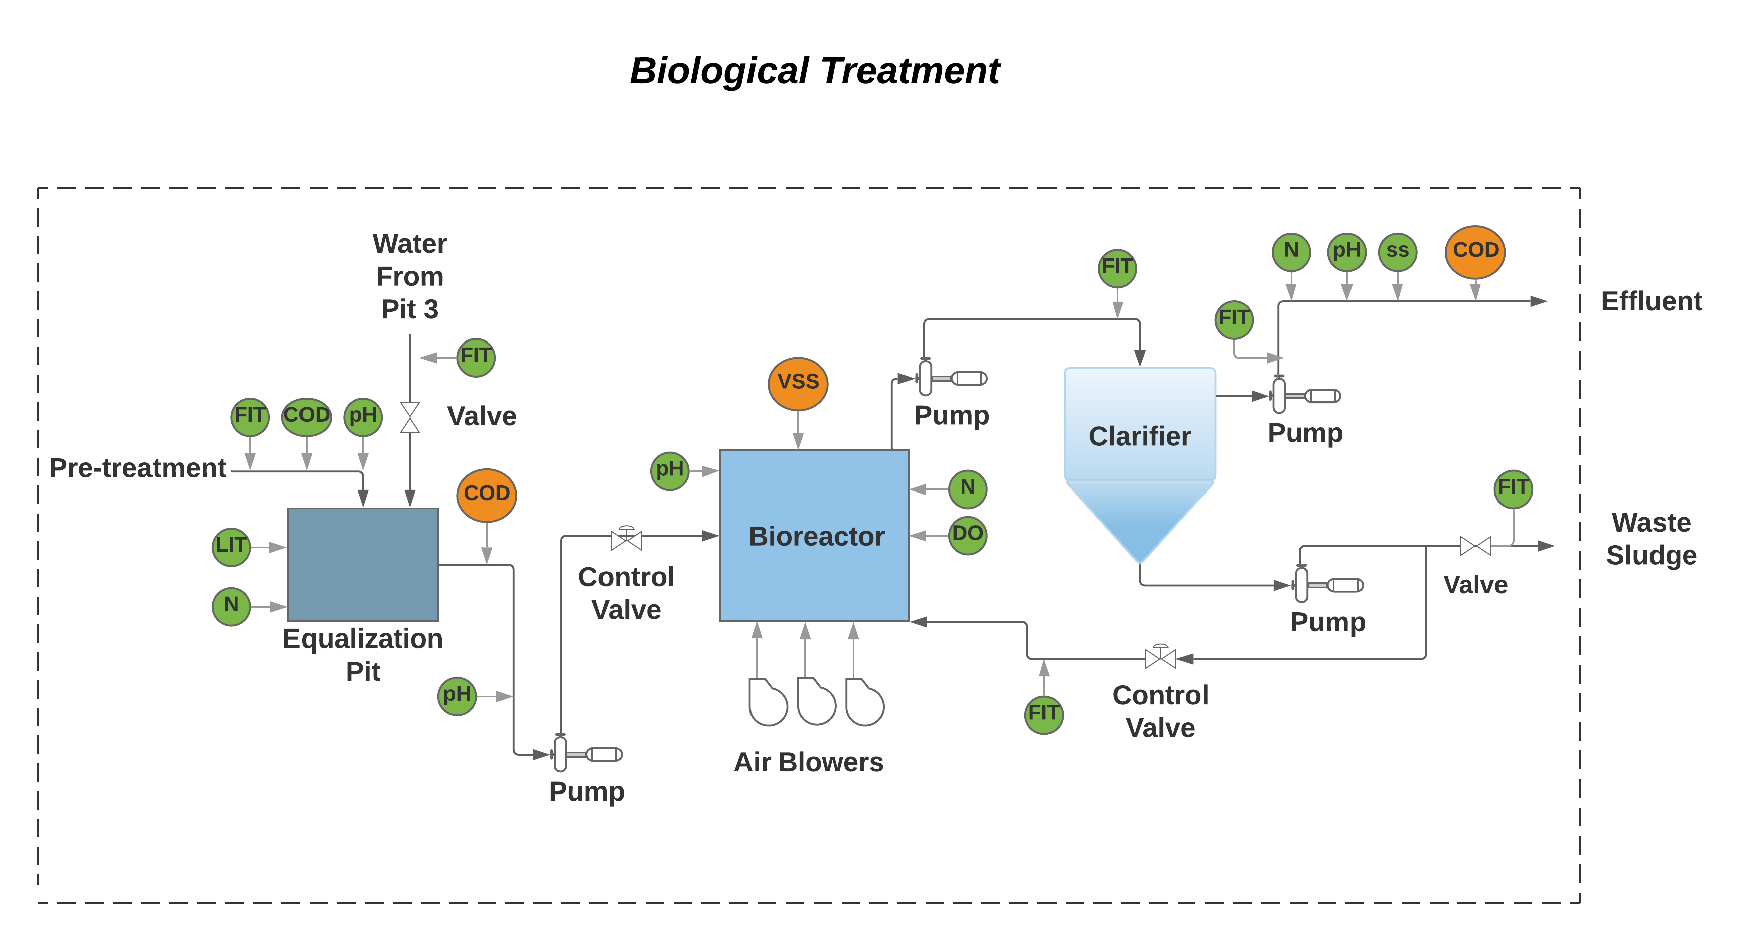
\includegraphics[width=\linewidth]{figures/Ch4/Biological-treatment-stage.pdf}
\caption{Biological Treatment Stage}
\label{f:Biological-treatment}
\end{figure}

\autoref{f:Biological-treatment} illustrates the composition of the biological treatment stage, which is the case of study in this research. This stage has three main components, and each one plays a vital role in the organic load removal; an equalization pit, a bioreactor, and a clarifier. Green circles represent measured variables of interest and potential input variables for the system. Orange circles are the target variables of this work, which are also available.

This work uses Python programming language to implement the intelligent system, supported by several libraries such as Numpy, Pandas, Tensor Flow, Sci-kit Learn, and Matplotlib, among others. A GitHub repository contains the files corresponding to code, models, and some of the results presented in this document \footnote{\url{https://github.com/carloscp3009/Machine-Learning-Approaches-for-Industrial-data-forecasting}}. 

The study utilizes 343 data samples from a wastewater treatment facility located in Nantong, China. Measurements correspond to most of the year 2018 and present a daily frequency, which experts consider accurate to capture the process dynamics. The measured variables of the process available for this work are:

\begin{itemize}
 \item	Flow (FIT)
 \item	COD of influent water
 \item	Suspended solids in influent water (SS)
 \item	Mixed liquor suspended solids (MLSS)
 \item	Mixed liquor volatile suspended solids (MLVSS)
 \item	Nitrogen (N)
 \item	pH
 \item	Mixed liquor dissolved oxygen (DO)
 \item	Food to microorganism (F/M)
\end{itemize}

The following nomenclature determines the unit process or component within the biological stage that the variable is measured.

\begin{itemize}
 \item	EQ = Equalizer
 \item	BIO = Bioreactor
 \item	BT\textsubscript{N}= Bioreactor Pit N
 \item	BT\textsubscript{C}= Bioreactor Pit C
 \item	Clari = Clarifier
 \item	OxT = Oxidation Tank
 \item	D = Discharge Pit
\end{itemize}

\section{Predictive model Approaches}
\label{s:model-design}
One of the first steps to build a data-driven system is to select which variables will feed the model. The correlation coefficient allows the selection of the exogenous variables used as inputs for the system. These selected variables enhance the model learning capability by reducing the noise of uncorrelated variables and decreasing the number of trainable parameters, which implies a model complexity reduction. 

After variable selection, the dataset is split into training (0.8) and testing (0.2) sets. The first 80\% of the dataset serves as examples for the model to learn. The other 20 \% is used to evaluate the performance of the model using new data, obtaining certainty of its behaviour in production mode. 

\begin{figure}[h]
\centering
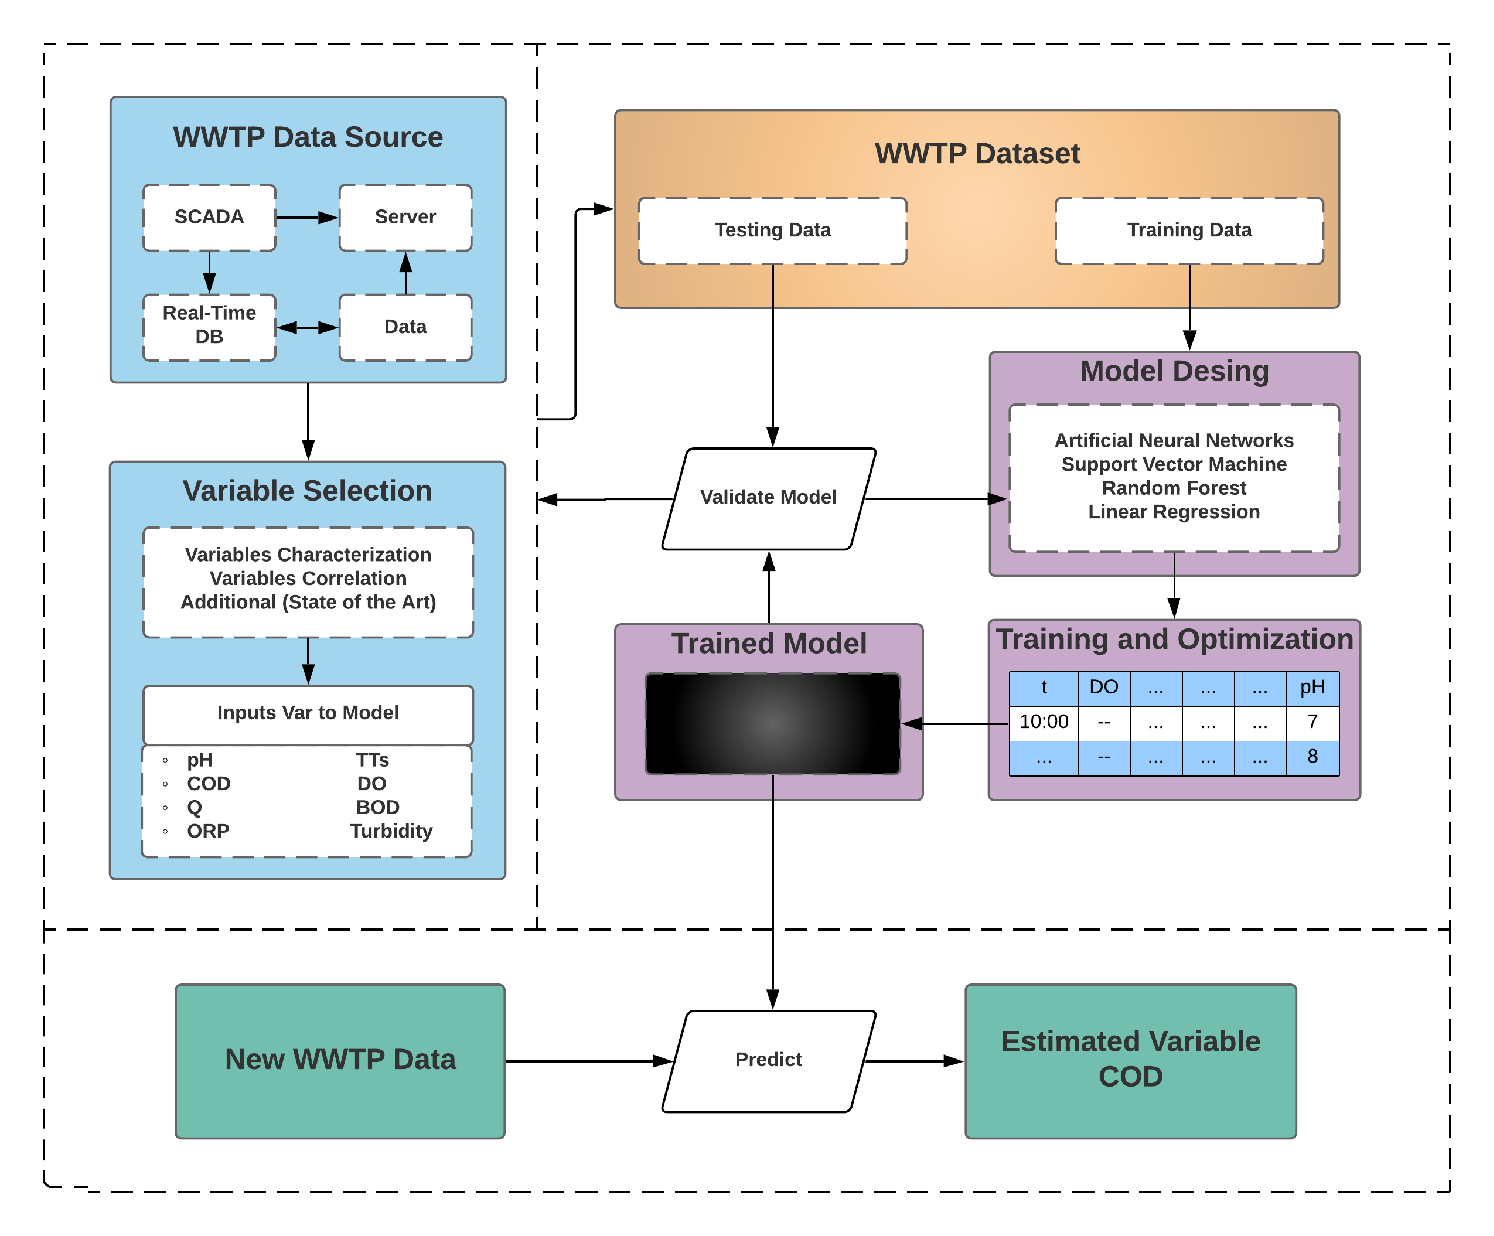
\includegraphics[width=\linewidth]{figures/Ch4/training-FlowChart.pdf}
\caption{Training flow chart}
\label{f:training-flowchart}
\end{figure}

Once a technique is selected, the training of the model begins. An error measurement is necessary to support the performance of the model. Therefore, the \ac{MAPE} is used as the evaluation metric for this study defined as shown in \autoref{eq:MAPE}.

\subsection{Approach 1}
\label{s:Approach1}

First, the target variable taken from the dataset is studied using a time-series decomposition technique that transforms and decomposes the variable into three additive components: trend, seasonality and residual. Leveraging an autocorrelation study, the first two components are estimated using their past values. On the other hand, the residual component is assessed using an \ac{FFNN}, which received exogenous variables selected from a correlation study and a past value of the same component. Finally, the addition of the three components provides the \ac{COD} prediction. \autoref{f:Approach 1} shows in more detail how the model is conceived and how forecasting is achieved.

\begin{figure}[h]
\centering
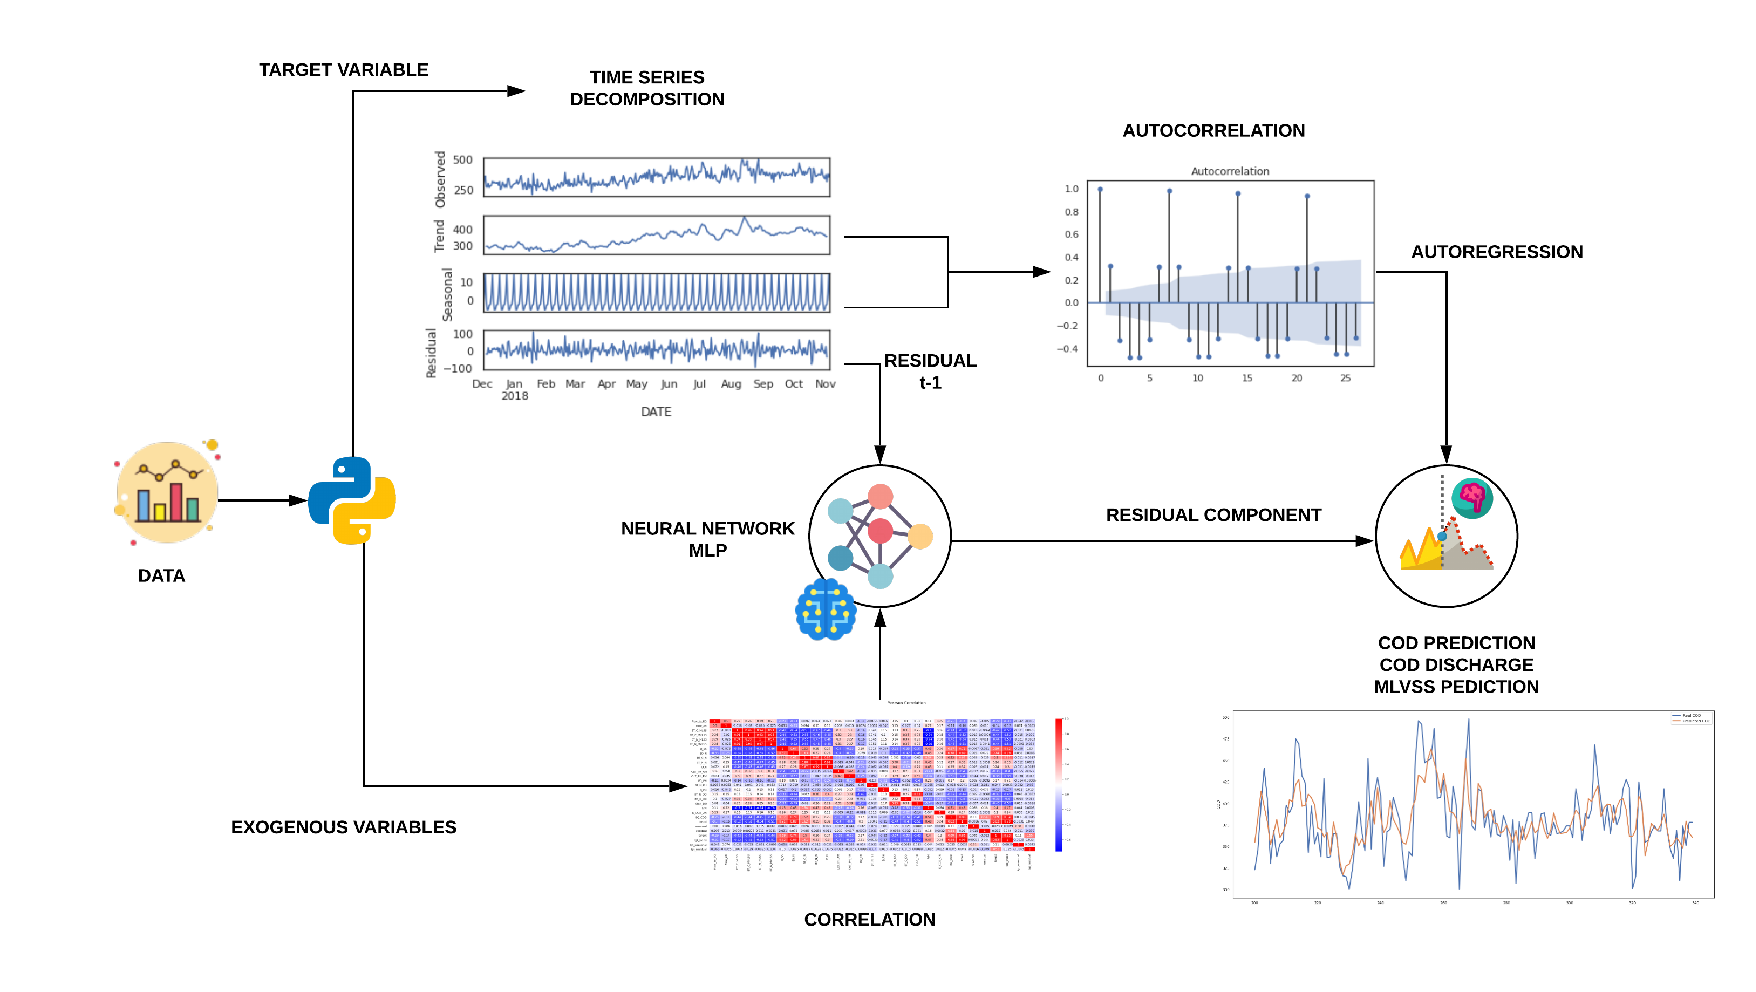
\includegraphics[width=\linewidth]{figures/Ch4/Approach1.pdf}
\caption{Approach 1}
\label{f:Approach 1}
\end{figure}

\subsubsection{Time Series Decomposition}
\label{ss:time-series-decomposition}

Time series decomposition is a time series analysis technique that allows splitting the target variable in trend, seasonality and residual components; the combination of these three components enables the reconstruction of the original variable \cite{Cryer2008}. This approach aims to forecast each component of the time series separately to obtain the target series using the additive model stated by Pearson and presented in \autoref{eq:time-series-decomposition}
\cite{dagum2010time}.

\begin{equation}\label{eq:time-series-decomposition}
    x_t = T_t + S_t + R_t
\end{equation}

\begin{itemize}
    \item \begin{math}X_t\end{math} is the observed time series.
    \item \begin{math}T_t\end{math} is the tendency or trend.
    \item \begin{math}S_t\end{math} is the seasonal movement.
    \item \begin{math}R_t\end{math} is the residual component.
\end{itemize}

\autoref{f:Time-series-decomposition} shows an example of how the equalizer’s COD decomposition looks like, where (a) shows the original COD variable, (b) the trend component, (c) the seasonal component and (d) the residual component.

\begin{figure}[h]
\centering
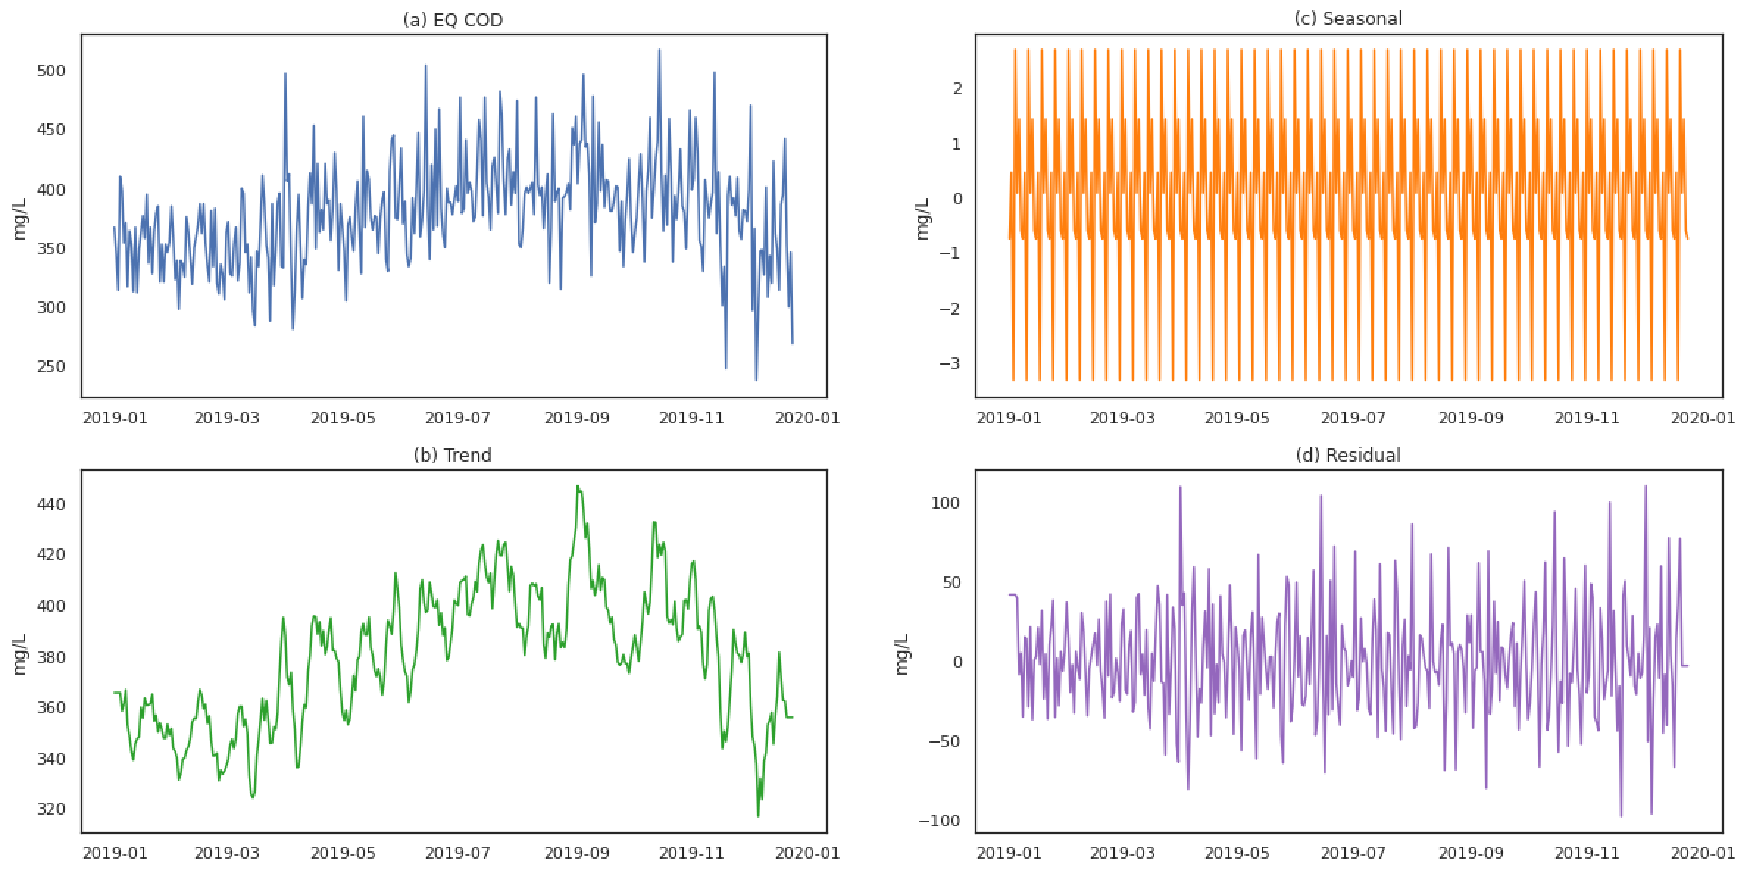
\includegraphics[width=\linewidth]{figures/Ch4/time_series_descompose.pdf}
\caption{Time Series Decomposition}
\label{f:Time-series-decomposition}
\end{figure}

\subsubsection{Autocorrelation Study}
\label{ss:autocorrelation}

After the time-series decomposition, both autocorrelation and partial autocorrelation studies were made on residual, seasonal and trend COD to extract the important characteristics. From this analysis, it was possible to conduct an autoregressive estimation of the trend and seasonal component of the series. \autoref{f:autocorrelation} shows the total and partial autocorrelation, respectively. The horizontal axis indicates the lagged time of the variable, and the vertical value the level of correlation with respect to the present value.

\begin{figure}[h]
\centering

    \begin{subfigure}{0.49\textwidth}
    \centering
    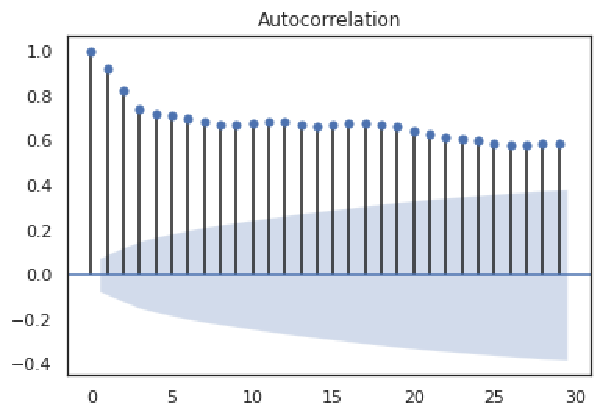
\includegraphics[width=\linewidth]{figures/Ch4/Trend_autocorr.pdf}
    \caption{ACF}
    \label{f:auto}
    \end{subfigure}
\hfill
    \begin{subfigure}{0.49\textwidth}
    \centering
    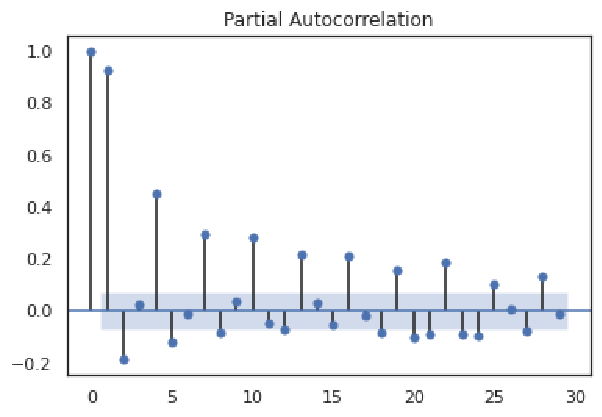
\includegraphics[width=\linewidth]{figures/Ch4/Trend_Partial_autocorr.pdf}
    \caption{PACF}
    \label{f:partial}
    \end{subfigure}

\caption{Autocorrelation study}
\label{f:autocorrelation}
\end{figure}

\subsection{Approach 2}
\label{s:Approach2}

The second approach uses a \ac{RNN}, specifically a \ac{LSTM}, a powerful network architecture for sequential data which considers the effect of past values of both endogenous and exogenous variables by itself and learns possible time patterns during the training. \autoref{f:Approach 2} shows a general overview of the second approach. This network requires some data pre-processing to structure the data in sequences format (seven past steps are considered for this study).

\begin{figure}[h]
\centering
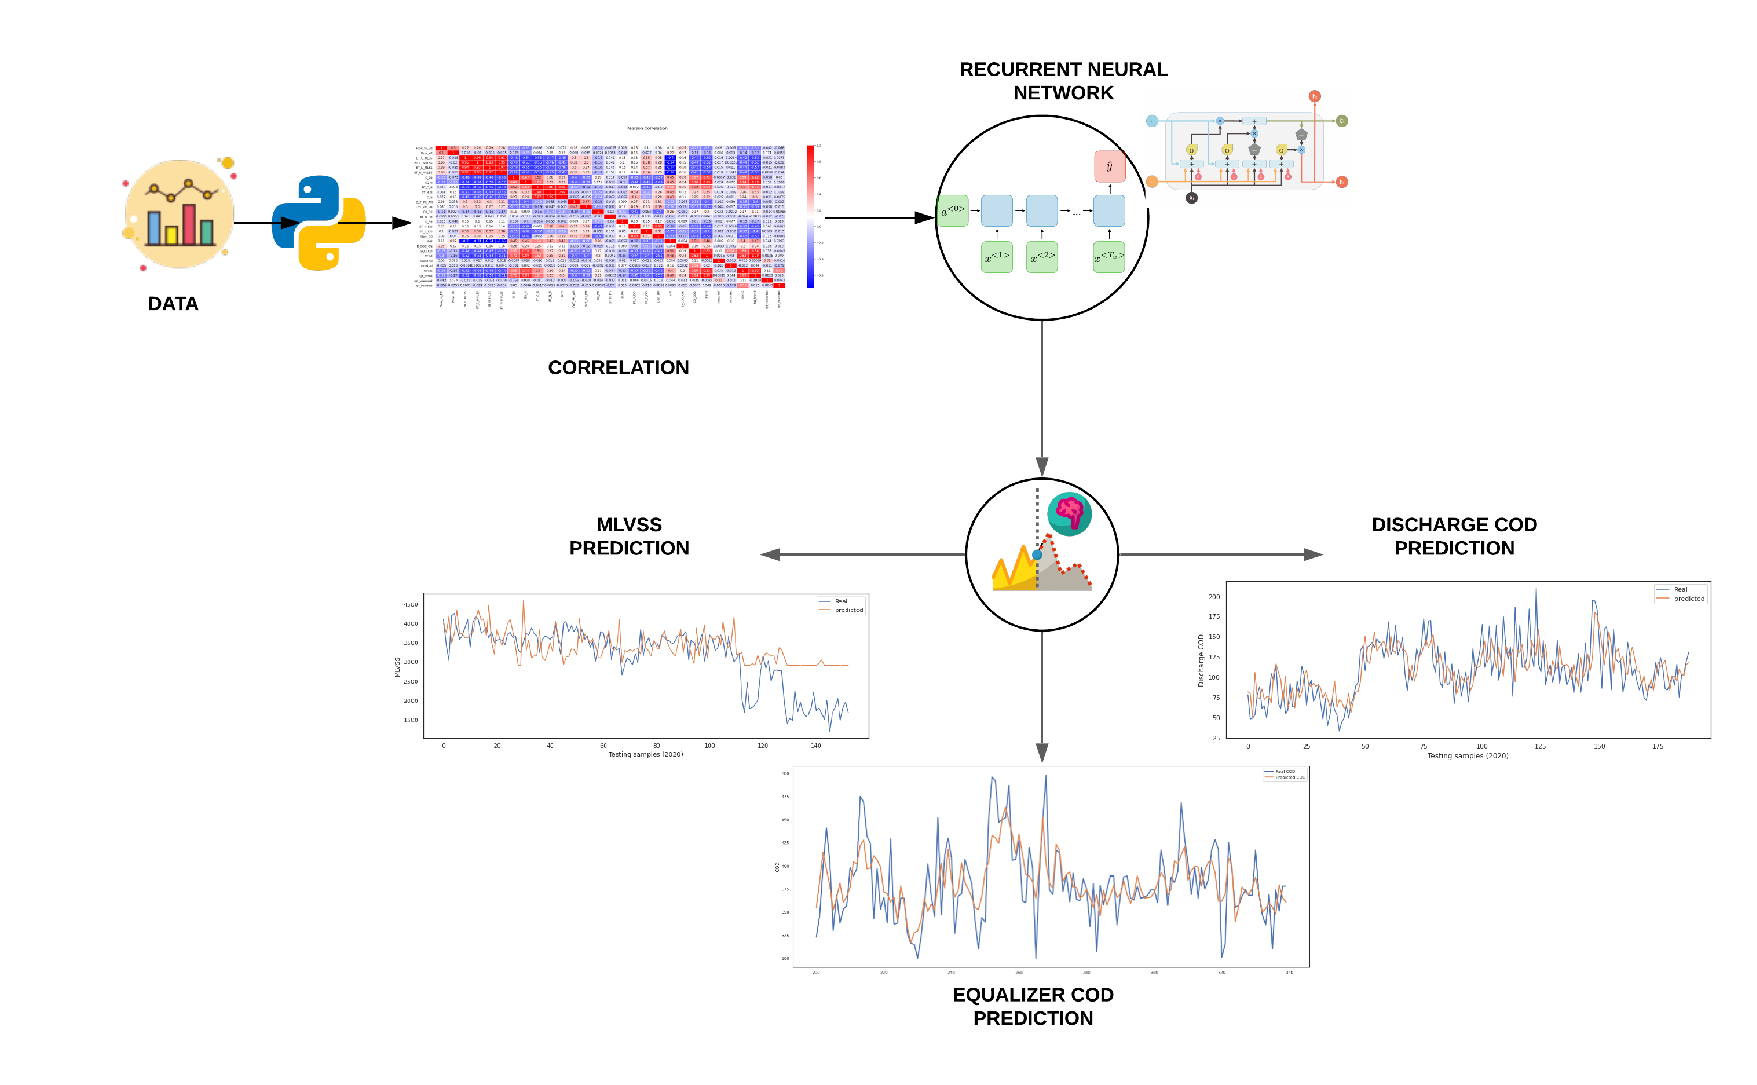
\includegraphics[width=\linewidth]{figures/Ch4/Approach2.pdf}
\caption{Approach 2}
\label{f:Approach 2}
\end{figure}

\subsection{Approach 3}
\label{s:Approach3}

The third approach proposed uses a machine learning technique based on Support Vector Machines. The \ac{SVR} algorithm offers an accurate prediction of the time series. This model receives as inputs the exogenous variables selected from the correlation analysis. The implemented model uses \ac{RBF} kernel, gamma of 0.001, epsilon equal to 0.2 and c value of 10.

\begin{figure}[h]
\centering
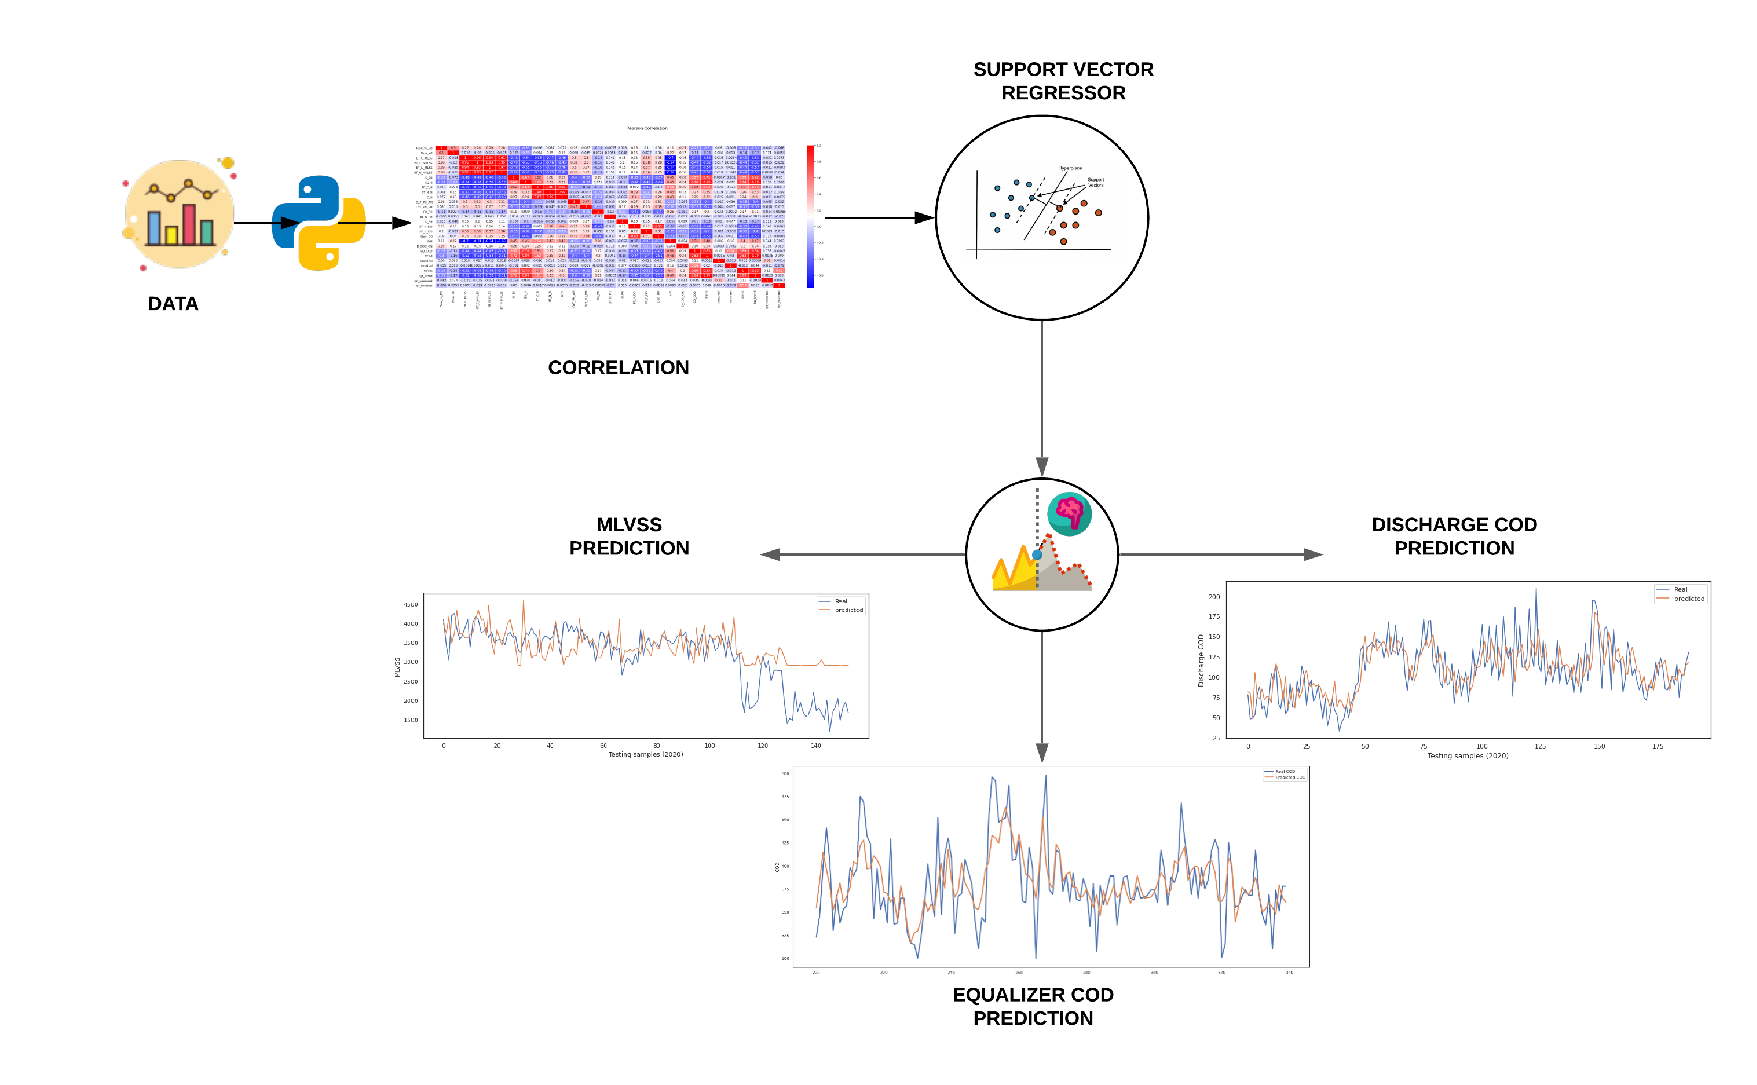
\includegraphics[width=\linewidth]{figures/Ch4/Approach3.pdf}
\caption{Approach 3}
\label{f:Approach 3}
\end{figure}

\section{Ensemble approaches to enhance single predictive models}
\label{s:Ensembles}

To enhance the prediction precision, an ensemble module is used to combine the output of each proposed approach. The purpose of different ensemble models is to take advantage of each model goodness and capability of recognizing different patterns in the data. Several theoretical and experimental studies show that combining different predictive methods results in a more robust model and presents better performance \cite{Nourani2021}. This ensemble module could use the pre-processed exogenous variables as inputs if needed.

Three different ensemble strategies are implemented and compared in this study. The final predictive system is presented in \autoref{f:Ensemble-approach} where the block diagram shows the models interaction needed in the system to achieve the final prediction. 

\begin{figure}[h]
\centering
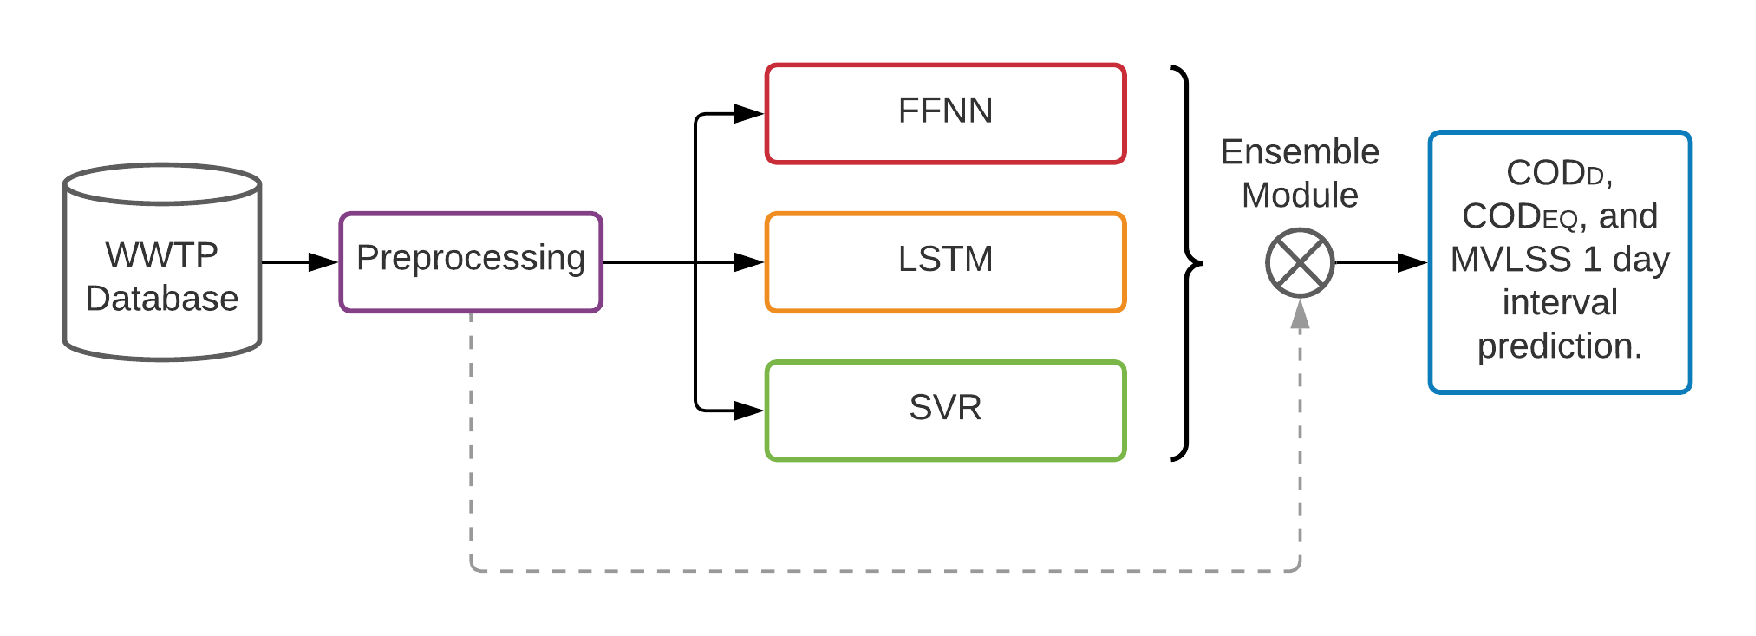
\includegraphics[width=\linewidth]{figures/Ch5/Thesis-Approaches-Ensemble.pdf}
\caption{Ensemble approach}
\label{f:Ensemble-approach}
\end{figure}

\subsection{Ensemble Approach 1}
\label{s:Ensemble-Approach1}
The first ensemble approach proposed is a simple averaging model obtained by calculating the mean of the single models' outputs. \autoref{eq:avg-ensemble} present the combination used in this approach. Since this average ensemble approach is one of the simplest combinations, it is considered the enhanced models' baseline. \autoref{f:Ensemble-approach1} illustrate how this ensemble works.

\begin{equation}\label{eq:avg-ensemble}
    \hat{Y} = \frac{1}{n} \sum_{i=1}^{n}  \hat{y}_i
\end{equation}

\begin{itemize}
    \item \begin{math}\hat{Y}\end{math} is the ensemble model prediction.
    \item \begin{math}n\end{math} is the number of models.
    \item \begin{math}\hat{y}_i\end{math} is each single model output.
\end{itemize}

\begin{figure}[h]
\centering
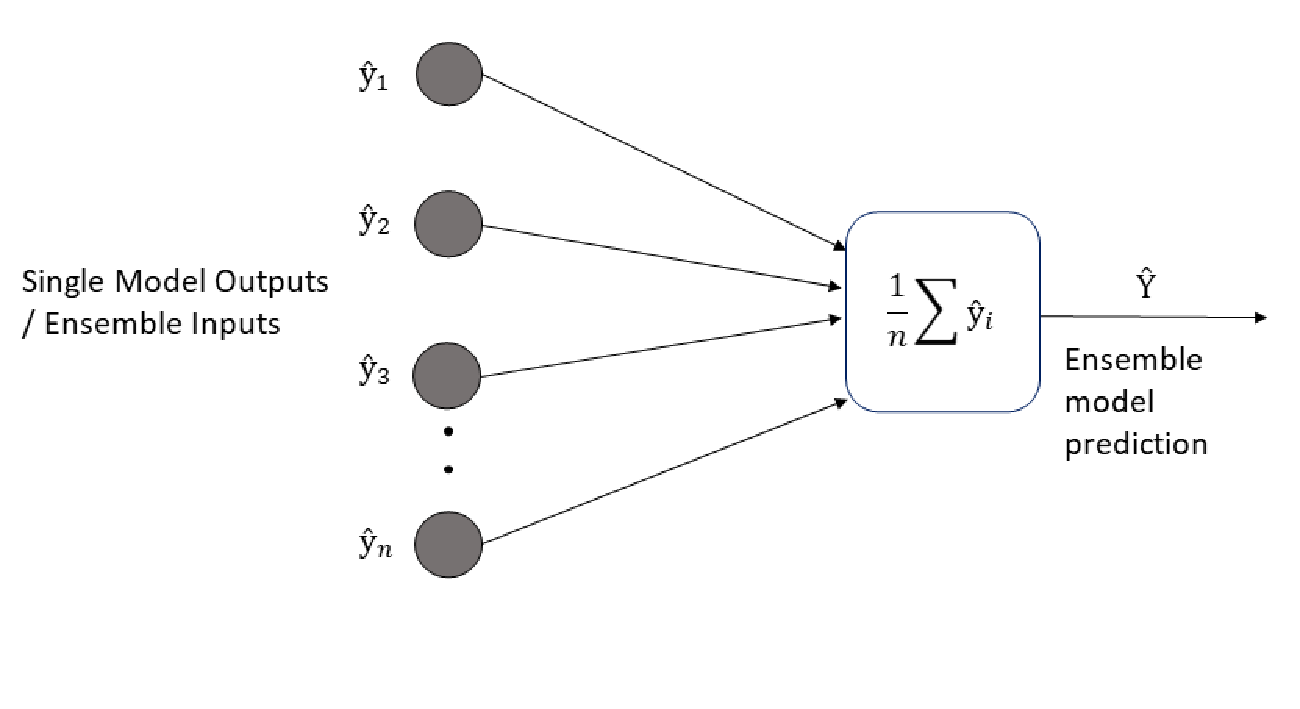
\includegraphics[width=\linewidth]{figures/Ch4/Ensemble_Approach1.pdf}
\caption{Average Ensemble approach}
\label{f:Ensemble-approach1}
\end{figure}

\subsection{Ensemble Approach 2}
\label{s:Ensemble-Approach2}
The second ensemble approach proposed uses a \ac{MLP} that receives as inputs; the single model outputs together with the same exogenous variables used to predict that target variable. The concept is that the \ac{ANN} finds a more complex but more accurate combination of the predicted results but also enhances the final prediction even more by using the exogenous variables. \autoref{f:Ensemble-approach2} shows how this ensemble approach is conceived. 

\begin{itemize}
    \item \begin{math}\hat{Y}\end{math} is the ensemble model prediction.
    \item \begin{math}n\end{math} is the number of models.
    \item \begin{math}\hat{y}_i\end{math} is each single model output.
    \item \begin{math}\hat{x}_i\end{math} is each exogenous variable selected previously for that target prediction.
    \item \begin{math}k\end{math} is the number of exogenous variables.
\end{itemize}

\begin{figure}[h]
\centering
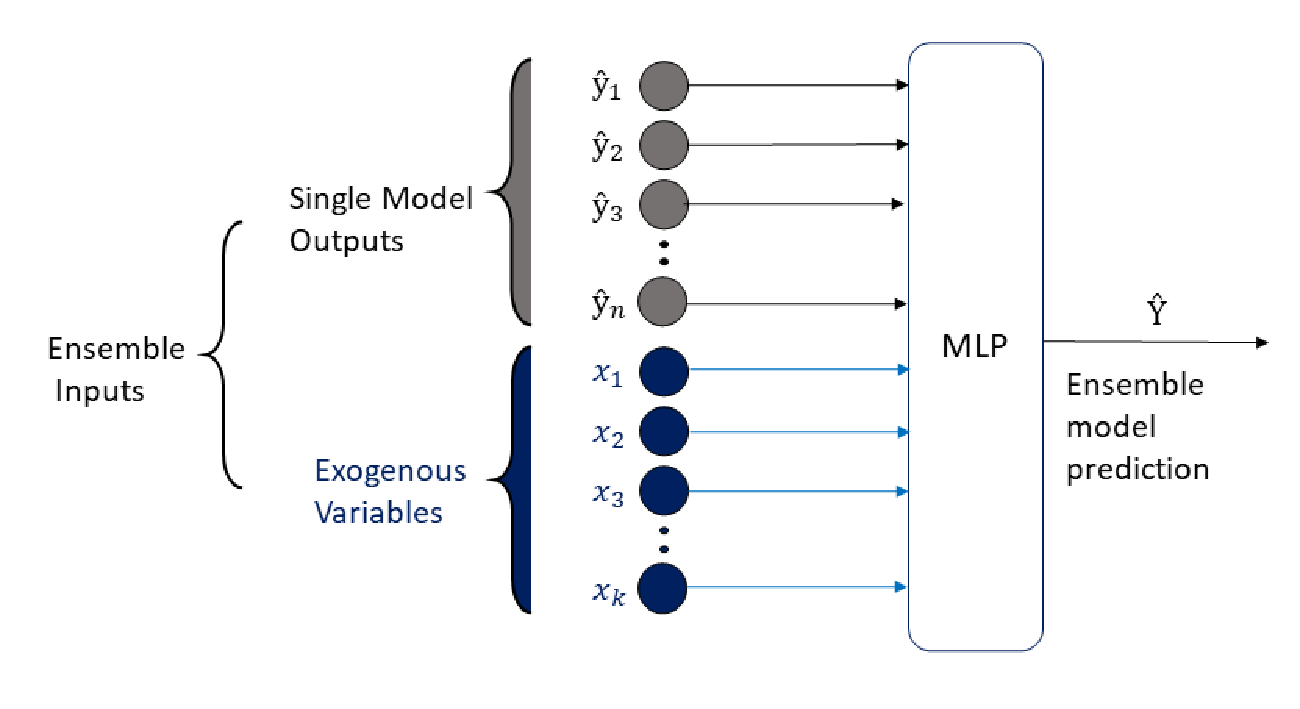
\includegraphics[width=\linewidth]{figures/Ch4/Ensemble_Approach2.pdf}
\caption{MLP Ensemble approach}
\label{f:Ensemble-approach2}
\end{figure}

\subsection{Ensemble Approach 3}
\label{s:Ensemble-Approach3}

\begin{figure}[h]
\centering
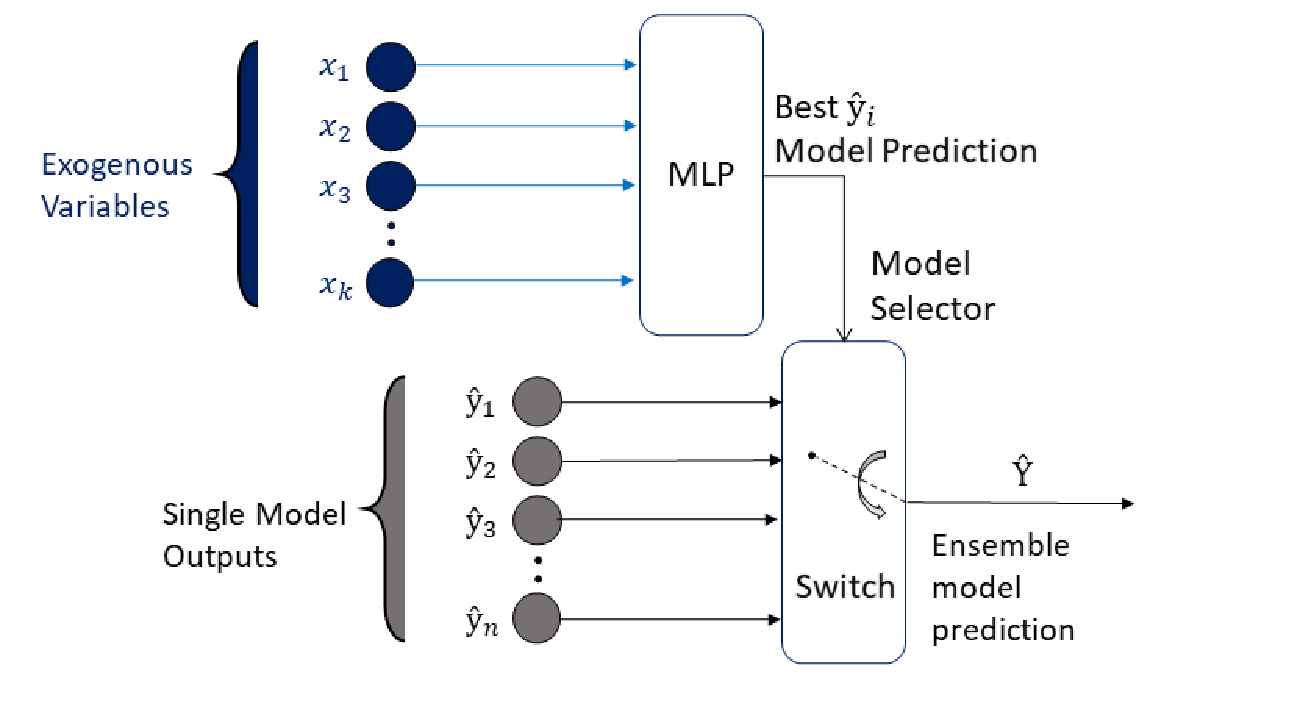
\includegraphics[width=\linewidth]{figures/Ch4/Ensemble_Approach3.pdf}
\caption{Selector Ensemble approach}
\label{f:Ensemble-approach3}
\end{figure}

The idea behind the last ensemble approach proposed is that each model performs better depending on the situation or the process conditions. An \ac{MLP} receives the exogenous variables which intend to represent or provide the information concerning the process state or conditions. The \ac{MLP} aims to estimate which model behaves the best in each time step. The absolute error between the expected output and the models' prediction is used to define which model performs the best at each sample and build a new dataset with the corresponding labels to train this classifier. 
The classifier prediction output is used to select the most suitable model to predict the target variable at the current time step. \autoref{f:Ensemble-approach3} shows how the Selection ensemble approach works.

\section{Summary}

\label{s:Contribution-1-Summary}

This chapter presents three approaches to predict time series variables of the wastewater treatment process. Also, three different ensemble approaches are proposed to enhance the intelligent system prediction performance.